\section{Results}

\subsection{Minikube Results}

After executing the commands in Listing~\ref{lst:minikube-cluster}, Minikube successfully creates a three-node cluster, comprising two worker nodes and one control plane node, as illustrated in Figure~\ref{fig:minikube-cluster}.

\begin{figure}[!htbp]
  \centering
  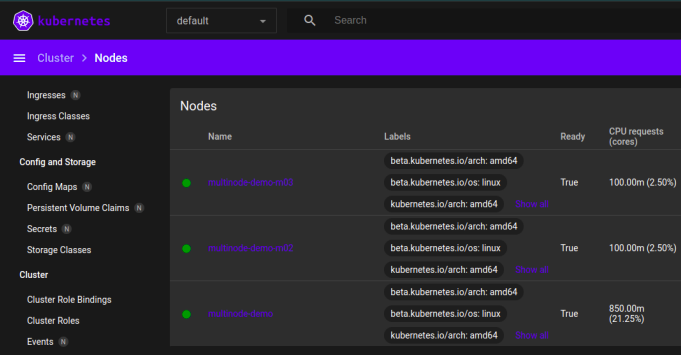
\includegraphics[width=0.45\textwidth]{figures/nodes.png}
  \caption{Minikube cluster with three nodes.}
  \label{fig:minikube-cluster}
\end{figure}

Following the execution of the commands in Listing~\ref{lst:kubectl_php_apache}, the PHP Apache server is deployed on the Minikube cluster.
The Kubernetes dashboard confirms the successful creation of the deployment and service, as depicted in Figures~\ref{fig:deployments} and~\ref{fig:services}, respectively.

\begin{figure}[!htbp]
  \centering
  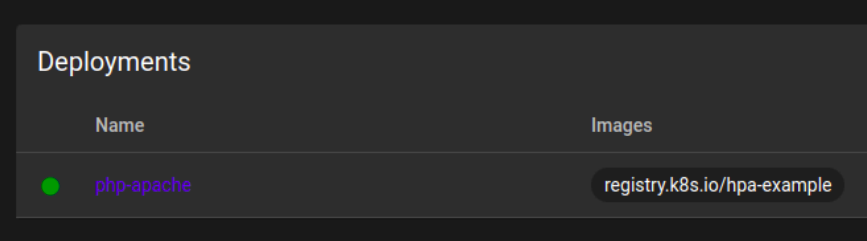
\includegraphics[width=0.45\textwidth]{figures/deployments.png}
  \caption{PHP Apache server deployment.}
  \label{fig:deployments}
\end{figure}

\begin{figure}[!htbp]
  \centering
  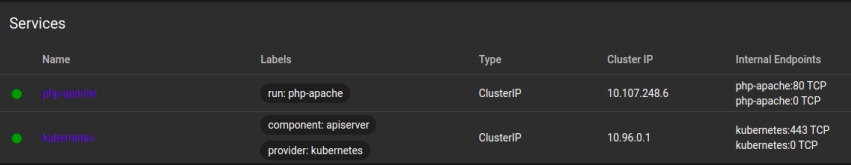
\includegraphics[width=0.45\textwidth]{figures/services.png}
  \caption{PHP Apache server service.}
  \label{fig:services}
\end{figure}

Next, the Horizontal Pod Autoscaler (HPA) is configured to scale the PHP Apache server deployment based on CPU utilization. A load test is then performed to artificially increase the CPU usage of the server. As shown in Figure~\ref{fig:hpa_increasing}, the HPA increases the number of replicas from one to four when CPU usage exceeds 50\%. In Figure~\ref{fig:hpa_max}, the HPA reaches its configured maximum of six replicas. Finally, after the load test is terminated, the CPU usage decreases, prompting the HPA to scale down the number of replicas from six to one, as illustrated in Figure~\ref{fig:hpa_decreasing}.

\begin{figure}[!htbp]
  \centering
  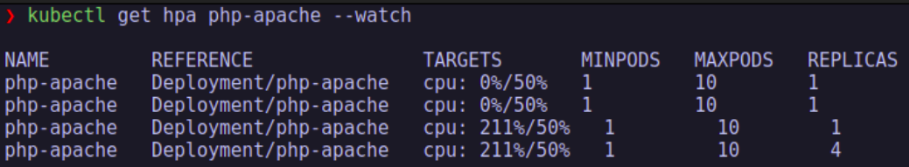
\includegraphics[width=0.45\textwidth]{figures/hpa_increasing.png}
  \caption{HPA increasing the number of replicas.}
  \label{fig:hpa_increasing}
\end{figure}

\begin{figure}[!htbp]
  \centering
  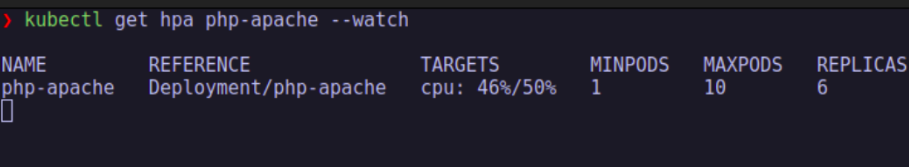
\includegraphics[width=0.45\textwidth]{figures/hpa_max.png}
  \caption{HPA scaling to the maximum number of replicas.}
  \label{fig:hpa_max}
\end{figure}

\begin{figure}[!htbp]
  \centering
  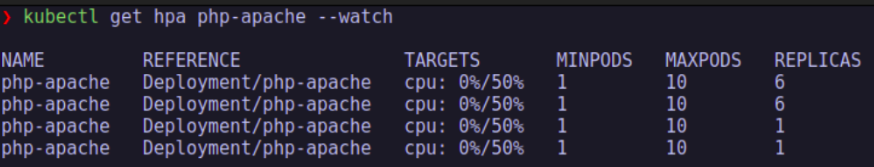
\includegraphics[width=0.45\textwidth]{figures/hpa_decreasing.png}
  \caption{HPA decreasing the number of replicas.}
  \label{fig:hpa_decreasing}
\end{figure}


\subsection{AWS EKS results}

After the execution of the commands to test the autoscaler, as outlined in Listing~\ref{lst:autoscaler-test}, The output of this command is presented in Figure~\ref{fig:metrics}.

\begin{figure}[!htbp]
  \centering
  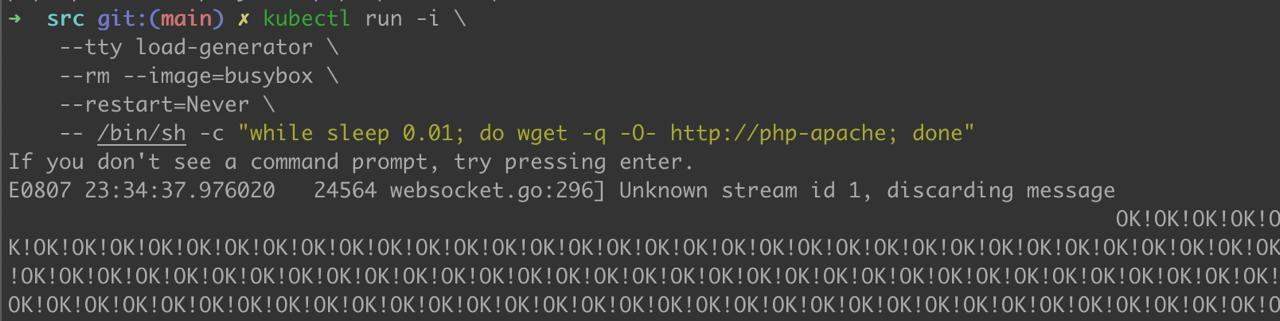
\includegraphics[width=0.45\textwidth]{figures/test-autoscaler.jpeg}
  \caption{Test autoscaler on EKS.}
  \label{fig:test-autoscaler}
\end{figure}

Next, we allowed approximately 2.5 minutes to elapse before proceeding with the command that displays the number of replicas managed by the autoscaler, as shown in Listing~\ref{lst:pods-number}. The output of this command is presented in Figure~\ref{fig:metrics}, where it is evident that nine replicas of the server were generated in response to the load induced by the test command.

\begin{figure}[!htbp]
  \centering
  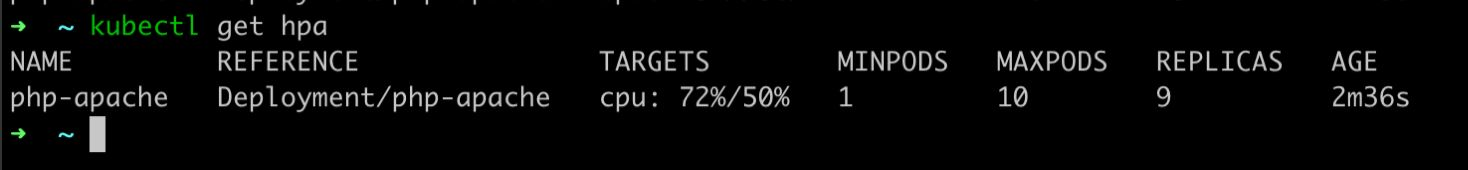
\includegraphics[width=0.45\textwidth]{figures/metrics.jpeg}
  \caption{PHP Apache server metrics.}
  \label{fig:metrics}
\end{figure}
